%%%% fs-run-time-motivation 

\subsection {Motivation}
\label{motivation-section}

Implementation of deterministic processing is tightly connected to system state management: if user-defined operations are pure functions and the total order is preserved, the processing becomes deterministic. Most of existing stream processing systems have been already supposing that user-defined operations are pure. Instead of providing a handler for external storage they give user operation the state object, provide the user an interface to change the state and finally store the resulting state object after the operation completes~\cite{carbone2015apache, apache:storm, Noghabi:2017:SSS:3137765.3137770}.

Let $B$ denote a business logic operation, $x, Y$ be input and output items, $h$, the state handler and $s_t$, the state object at time $t$. The change in contract is illustrated in (\ref{flink-contract}). In modern setting $B$ becomes stateless and state management is done on the system side. This change allows the system to implement fault tolerance mechanisms, but it also opens the opportunity to implement deterministic processing.

\begin{equation}
  \label{flink-contract}
  B(x, h) = Y \qquad\Longrightarrow\qquad B(x, s_{t}) = (Y, s_{t+1}) 
\end{equation}

The only difference between a state object $s_t$ and the other items in the stream is that state objects are produced, updated and consumed by the same operation. If a system allows cyclic execution graphs~\cite{Murray:2013:NTD:2517349.2522738} this difference becomes obsolete, as we can transfer state object from operations output to its input. We treat state object as a part of the stream and we call it {\it drifting state}. Drifting state allows moving fault tolerance logic from user-defined operations to common stream consistency mechanisms.

The second property of the system needed for deterministic processing is total order preservation. This one is quite challenging due to asynchronous nature of the network. On the other hand, we need to care about the order only in the operations that are order-sensitive. All stateless operations are tolerant to the out-of-order items. The more stateless operations we have, the easier the task becomes. Another important note is that calculations are partitioned, and order between items from different partitions does not influence the result. Partition could be calculated at single compute unit, which allows us to implement ordering within single unit instead of system-wide.

Taking into account above considerations we think that modern stream processing problem setup allows us to build a system that is able to provide deterministic processing with low performance overhead. The desired system properties are:
\begin{itemize}
  \item Computational model should be deterministic by design, i.e., it should produce deterministic results for any pipelines and business logic.
  \item The performance overhead should be low in comparison with the existing systems.
\end{itemize}
We will use the following principles for our system:
\begin{itemize}
  \item Support cyclic execution graph
  \item Localize state management in terms of system operation type
  \item A data partition must be processed on a single node
  \item MapReduce completeness
\end{itemize}

\subsection {Computational model}
%%%% fs-run-time-data-flow 
\label{model-section}

Data stream is a sequence of discrete events described by data items, internally represented as $(Payload, Meta)$. The $Payload$ is processed by a user-defined code, while the primary purpose of the meta-information is to impose the total order on data items. The $Meta$ is assigned at the entry (called {\em front}) and is discarded at the {\em barrier} just before the exit. 

The stream processing is specified by a logical execution graph. Each node of the graph represents a single operation on data items, and edges describe the routing of data items between operations. Our model allows cycles in the graph while such graphs are commonly assumed to be acyclic (DAGs) ~\cite{Zaharia:2016:ASU:3013530.2934664, Carbone:2017:SMA:3137765.3137777}. The cycles are required for specification of certain computations (e.g. MapReduce-based) with our set of operation types (outlined below). Figure~\ref{logical-graph-figure} shows the example of logical execution graph.

A distributed hardware environment is modeled as a set of {\em worker} processes. Each worker executes logical execution graph and has an assigned range of hash values used for physical routing of data items to workers. Each operation entry has a user-provided hash function called {\it balancing function}. This function is applied to the payload of data items and determines partitioning before each operation. After that, the data items are sent to the worker, which is responsible for the associated hash range. Therefore, load balancing explicitly depends on the user-defined balancing functions. 

% \begin{figure}[t]
%   \centering
%   \begin{minipage}[b]{.5\textwidth}
%     \centering
%     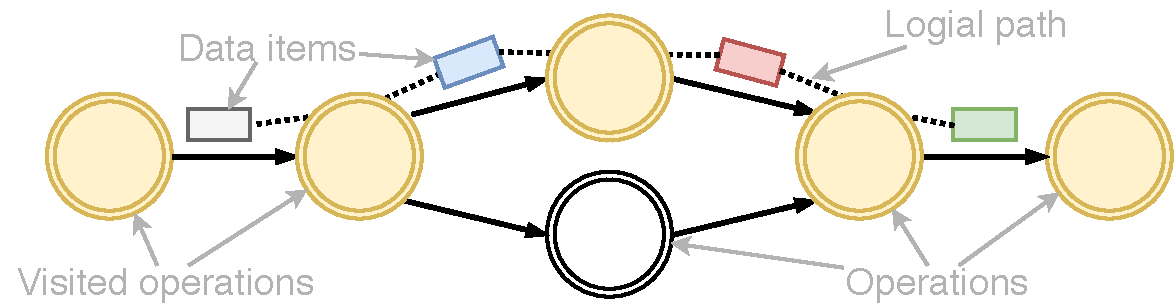
\includegraphics[width=0.9\linewidth]{Chapters/DeterministicModelRuntime/pics/logical-graph.pdf}
%     \caption{A logical execution  graph}
%     \label{logical-graph-figure}
%   \end{minipage}%
%   \begin{minipage}[b]{.5\textwidth}
%     \centering
%     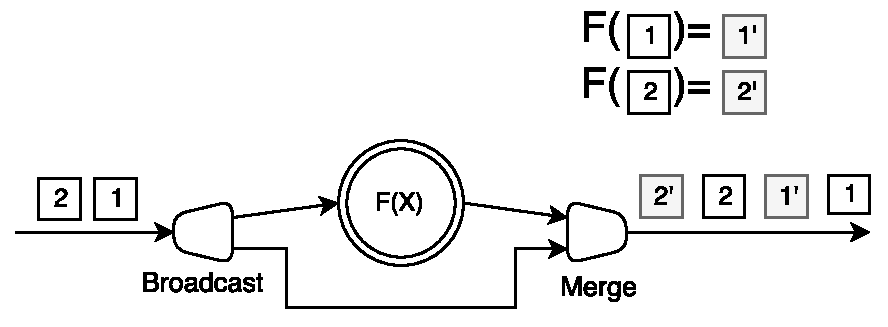
\includegraphics[width=\linewidth]{Chapters/DeterministicModelRuntime/pics/ordering}
%     \caption{The ordering model}
%     \label{ordering}
%   \end{minipage}
% \end{figure}

\begin{figure}[t]
  \centering
  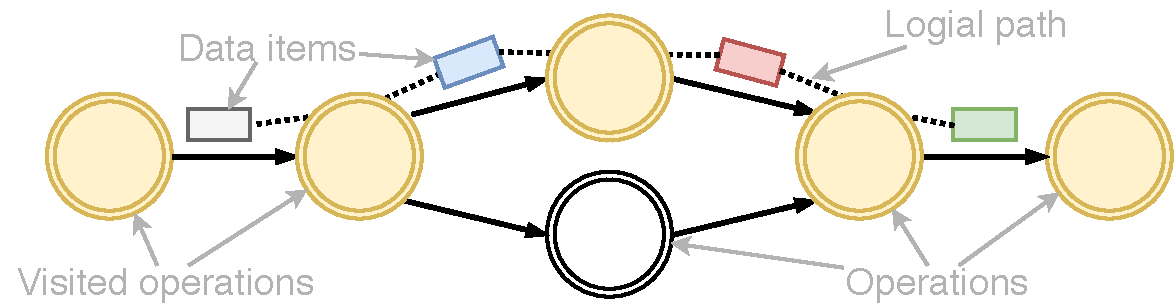
\includegraphics[width=0.8\textwidth]{Chapters/DeterministicModelRuntime/pics/logical-graph.pdf}
  \caption{A logical execution  graph}
  \label{logical-graph-figure}
\end{figure}

\begin{figure}[t]
  \centering
  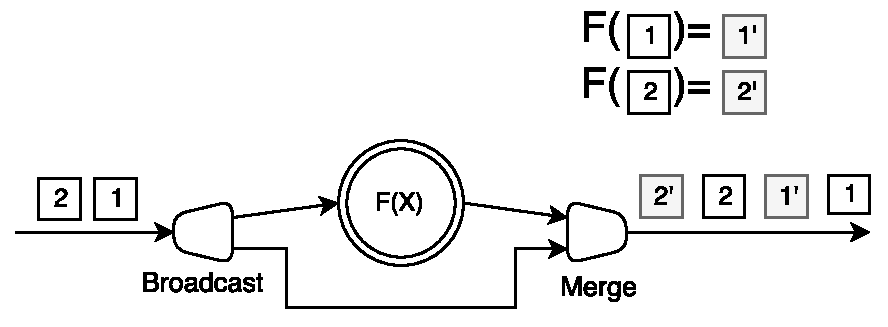
\includegraphics[width=0.7\textwidth]{Chapters/DeterministicModelRuntime/pics/ordering}
  \caption{The ordering model}
  \label{ordering}
\end{figure}

Data items are totally ordered according to labeles assigned to events at the entry as a part of meta-information. All operations preserve this order. Any additional items produced by an operation are placed between the item being processed and the next item. The ordering labels are dropped when items are delivered from the barrier. 

The ordering is illustrated  in Figure~\ref{ordering}. Data item with payload $1'$ is the derivative of the item with payload $1$, according to operation $F$. The same is for items with payloads $2'$ and $2$. After merge operation, the order between $1$ and $2$ is preserved. Furthermore, $1'$ follows $1$, and $2'$ follows $2$.  


The list of available operations includes:
\begin {description}
  \item [Map] applies a user-defined function to the payload of an input item and returns a (possibly empty) sequence of data items with transformed payloads. 

  \item [Broadcast] replicates an input item to the specified number of operations.

  \item [Merge] operation is initialized with the specified number of input nodes. It sends all incoming data to the output.

  \item [Grouping] constructs a single item containing a set of consecutive items that have the same value of partition function. The maximum number of items that can be grouped is specified as a parameter  $Window Size$. 
    
  The output item of the grouping has the same ordering label as the last item in the output group. Groupings of different partitions are independent. Grouping is the only operation that has a state.
\end {description}

The following example illustrates  the grouping operation. Let the input stream be a series of integers: $ 1,2,3, \ldots$, and the  partition function returns for even numbers and 0 otherwise. If the window is set to 3, the output is 
$$(1), (2), (1|3), (2|4), (1|3|5), (2|4|6), (3|5|7), (4|6|8), \ldots$$


\subsection{State updates}
\label{fs-drifting}

An important special case of grouping with $Window Size = 2$  provides for realization of stateful calculations with drifting state technique manifested in section~\ref{motivation-section}. Indeed, consider a map operation that follows the grouping and sends its output to the grouping input. This map operation receives a pair of its previous output considered as the state object, and new incoming item from the source stream. The map operation calculates new state object and sends it back as the grouping input. 

As an example, let us demonstrate a generic MapReduce transformation. The map stage of MapReduce can be expressed in terms of our map operation. The generic reduce stage can be presented as

\begin {tabbing}
1234\=1234\= \kill
{\bf for} $mapped \in values$ {\bf do}   \\
\>$accumulator$ := combine ($mapped$, $accumulator$); \\
{\bf end for} \\
{\bf return } $accumulator$;
\end {tabbing}

The {\it accumulator} is an explicit state that should be kept between subsequent iterations. To implement reduce stage we apply the drifting state technique and make the accumulator value a part of the stream. Figure~\ref{mapreduce-graph-figure} shows a generic graph for the MapReduce transformation. Map and reduce stages are highlighted with a dashed line. 

\begin{figure}[t]
  \centering
  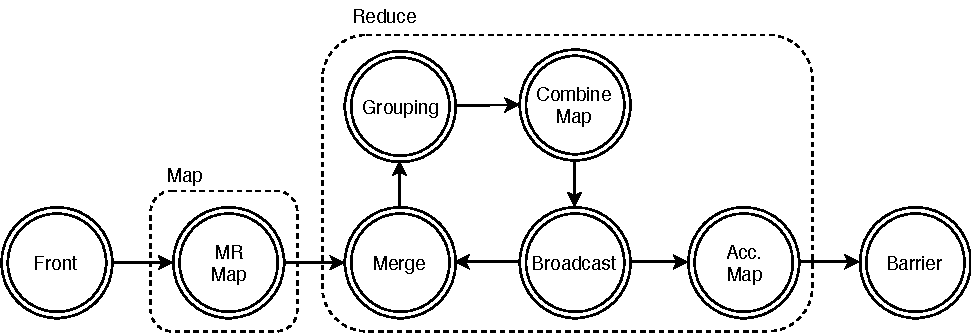
\includegraphics[width=0.8\textwidth]{Chapters/DeterministicModelRuntime/pics/mapreduce}
  \caption{Logical graph for MapReduce transformations}
  \label {mapreduce-graph-figure}
\end{figure}

There are four types of data items in this stream: {\em input}, {\em mapped}, {\em accumulator}, and {\em reduced}. The operations of the stream have the following purposes:

\begin{itemize}
  \item The first map operation outputs mapped items according to map stage of MapReduce model.
  
  \item The grouping with $WindowSize=2$ groups the $accumulator$ with next $mapped$ item. 
  
  \item The combine map produces a new state of $accumulator$ to be sent to grouping.
  
  \item The final map converts $accumulator$ into final reduce output.
\end{itemize}

Ordering rules  guarantee that each $accumulator$  item always arrives at the grouping right before next not yet combined mapped item. The cycle gives the ability for new accumulator items to get back in the grouping operation. Thereby, the stream reacts to each input item by generating new reduced item, which contains the actual value of the reduce stage.

\subsection {Deterministic computation}
\label {fs-collision} 

To restrict outputs to only one possible result, we impose the following  restrictions on our model: 

\begin{itemize}
  \item We require map function to be pure: return value is only determined by its input values, without observable side effects
  \item We impose a strict ordering requirement on the grouping  input
\end{itemize}

While the former can be satisfied by moderating the  business logic, the latter is foreign to the distributed systems: it is hard to ensure the right order of delivery due to asynchrony inherent for a distributed system. There are two most common methods that are used to implement order-sensitive operators: in-order processing (IOP)~\cite{Arasu:2006:CCQ:1146461.1146463, Cranor:2003:GSD:872757.872838} and out-of-order processing (OOP)~\cite{Li:2008:OPN:1453856.1453890}. According to IOP approach, each operation must enforce the total order on output elements. This method does not scale well, because it requires buffering before each, even stateless, operation within pipeline until the total order is reached~\cite{Li:2008:OPN:1453856.1453890}. OOP is an approach that does not require order maintenance if it is not needed. In the case of ordering requirements, OOP buffers input items until a special condition is satisfied. This condition is based on progress indicators such as punctuations~\cite{Tucker:2003:EPS:776752.776780}, low watermarks~\cite{Akidau:2013:MFS:2536222.2536229}, or heartbeats~\cite{Srivastava:2004:FTM:1055558.1055596}.  

Some state-of-the-art stream processing systems adopt OOP~\cite{Carbone:2017:SMA:3137765.3137777}, but they suppose that items must be buffered before each order-sensitive operation if deterministic results are required. In our system, we use an optimistic approach for handling out-of-order items, that is based on OOP, but require single buffer per computational pipeline, no matter how many stateful operations it contains.

Only the grouping operation retains a dependency on the order of incoming items. Within the  optimistic approach, we accept the fact that grouping can produce incorrect output, but we guarantee that all correct groups are eventually produced. To eventually produce all correct tuples, we use an approach called {\it repair}. If an item preceding already processed items arrives at the grouping operation, all items starting with the just arrived one are re-processed, and {\em tombstones} (invalidator) are generated for all items produced earlier for all input items processed before the new one. A tombstone for an item is the same item marked with a flag in its meta-information. Hence, it traverses over the same physical path as the invalidated item.

An example of grouping repair is shown in Figure~\ref{grouping-replaying}. The green item is out-of-order. The output consists of the new valid items  $(1, 2)$ and $(2, 3)$  and the tombstone $(1, 3)_{tomb}$ for the previously generated item.

\begin{figure}[t]
  \centering
  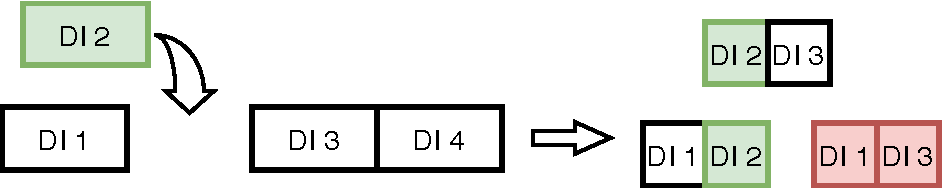
\includegraphics[width=0.6\textwidth]{Chapters/DeterministicModelRuntime/pics/grouping-replaying}
  \caption{The repair in grouping with $WindowSize = 2$.}
  \label {grouping-replaying}
\end{figure}

The barrier  keeps outgoing items on hold and filters out invalid elements, when corresponding tombstones arrive. As soon as no tombstones preceding certain point cannot arrive anymore, items are delivered  up to this point. More details can be found  in section~\ref{fs-impl}.

